%
%

%%-----------------------------------------------------
%%-----------------------------------------------------
\section{Televiéndonos}

%%-----------------------------------------------------
\begin{frame}
\frametitle{Jitsi}

\begin{columns}[T]
\begin{column}{.48\textwidth}

\includegraphics[width=6.5cm]{figs/jitsi-logo}

\begin{flushright}
  {\Large
    \url{http://meet.jitsi.org}
  }
\end{flushright}

\end{column}%
\hfill%
\begin{column}{.50\textwidth}
{\Large
\begin{itemize}
\item Conjunto de herramientas libres para videoconferencia
\item Funciona desde navegador y app en móvil
\item Herramientas modulares, pueden componerse de muchas forams
\item Permite integración con otros servicios (streaming, almacenamiento...)
\end{itemize}
}
\end{column}%
\end{columns}

\end{frame}


%%-----------------------------------------------------
\begin{frame}
\frametitle{Herramientas}

{\Large
  
  \begin{itemize}
  \item Jitsi Videobridge: servidor puente para videoconferencia
  \item Jitsi Meet: app JavaScript sobre WebRTC
  \item jigasi: pasarela a SIP
  \item jicofo: gestión de sesión en conferencias
  \item jibri: grabación / streaming
  \end{itemize}
  
}
\end{frame}


%%-----------------------------------------------------
\begin{frame}
\frametitle{Características}

{\Large
  
  \begin{itemize}
  \item Canales de video y audio sin mezclado en servidor
  \item Menos latencia, mejor escalabilidad en infraestructura
  \item WebRTC: basta un navegador
  \item Gestión avanzada de video en servidor
  \item Infraestrctura fácil de desplegar (Debian, Ubuntu)
  \end{itemize}
  
}
\end{frame}

%%-----------------------------------------------------
\begin{frame}

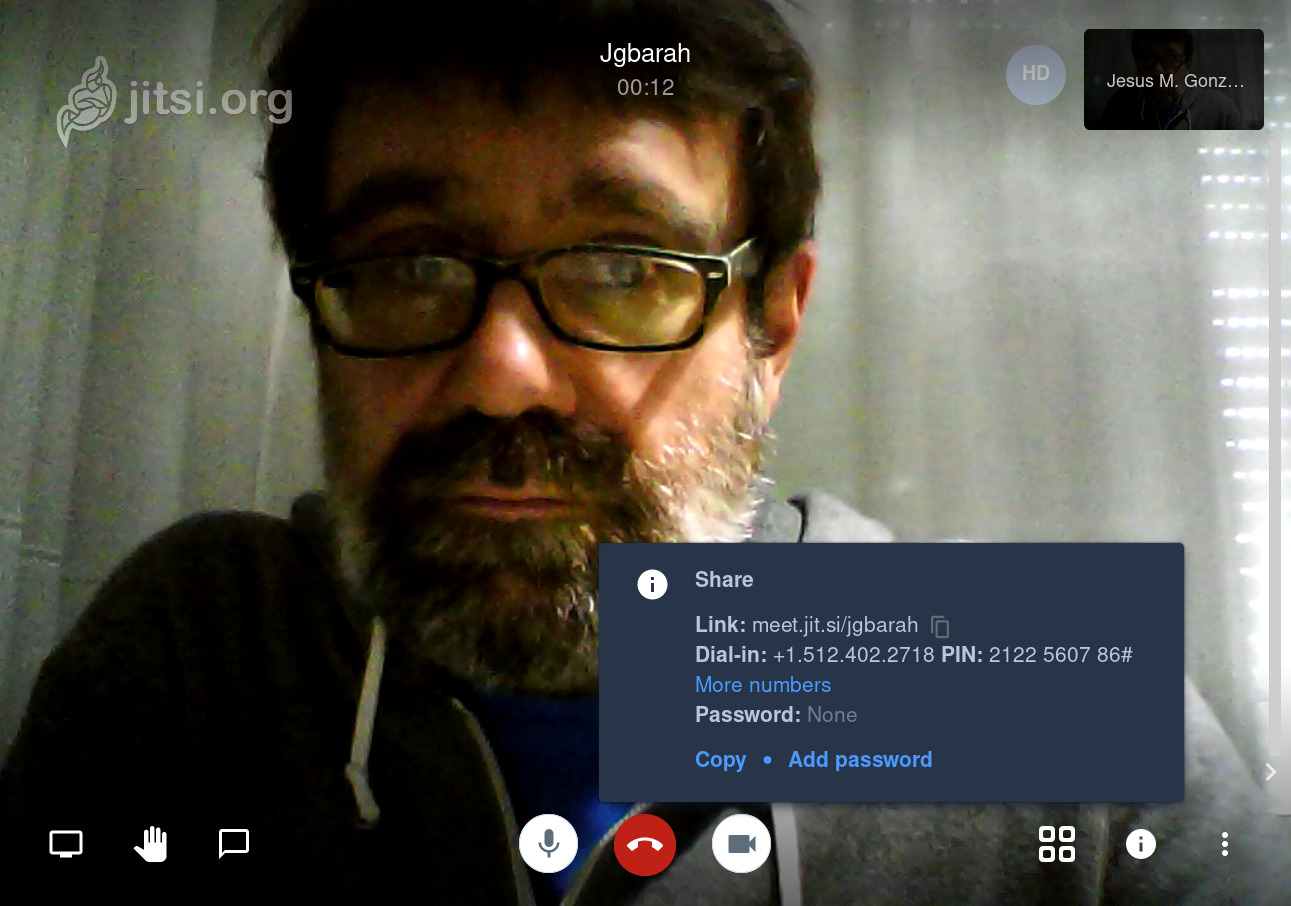
\includegraphics[width=11.5cm]{figs/jitsi-captura} 

\end{frame}


\end{frame}






